\documentclass{article}
\usepackage[T1]{fontenc}
\usepackage[utf8]{inputenc}
\usepackage[margin=1in]{geometry}
\usepackage{fancyhdr} 
\usepackage{listings}
\usepackage[ruled,vlined]{algorithm2e}
\usepackage{amsthm}
\usepackage{amsfonts}
\usepackage{amssymb}
\usepackage{graphicx}
\usepackage[dvipsnames]{xcolor}
\usepackage{xy}
% \usepackage{url} % Commented out because hyperref provides similar functionality
\usepackage{parskip}
\usepackage{comment}
\usepackage{setspace}
\usepackage{enumerate}
\usepackage{multirow}
\usepackage{hyperref}
\usepackage{caption}
\usepackage{subcaption}
\usepackage{booktabs}
\usepackage{wrapfig}
\usepackage{times}

\captionsetup[figure]{font={small,it}}

\usepackage[backend=biber,style=numeric,sortcites,maxbibnames=99]{biblatex}
\addbibresource{references.bib}

\newcommand{\HRule}{\rule{\linewidth}{0.5mm}}
\newcommand{\Hrule}{\rule{\linewidth}{0.3mm}}
\newcommand{\classnum}{CS-GY 6313 B}

\makeatletter% since there's an at-sign (@) in the command name
\renewcommand{\@maketitle}{%
  \parindent=0pt% don't indent paragraphs in the title block
  \centering
  {\Large \bfseries\textsc{\@title}}
  \HRule\par%
  \textit{\@author \hfill \classnum}
  \par
}
\makeatother% resets the meaning of the at-sign (@)

\title{Assignment \#2: Misleading Visualization}

\author{Ivan Aristy}
% \classnum

\begin{document}
  \maketitle % prints the title block
  \thispagestyle{empty}
  % \vspace{-15pt}

\section{Visualizations}
\label{sec:sec1}

The following are the two Visualizations that I have created for this Assignment, 
please note that the earnest visualization has elements that define its "earnestness",
ommited as per the assignment's obfuscation mandate.

% \begin{figure}[ht] 
%   \centering
%   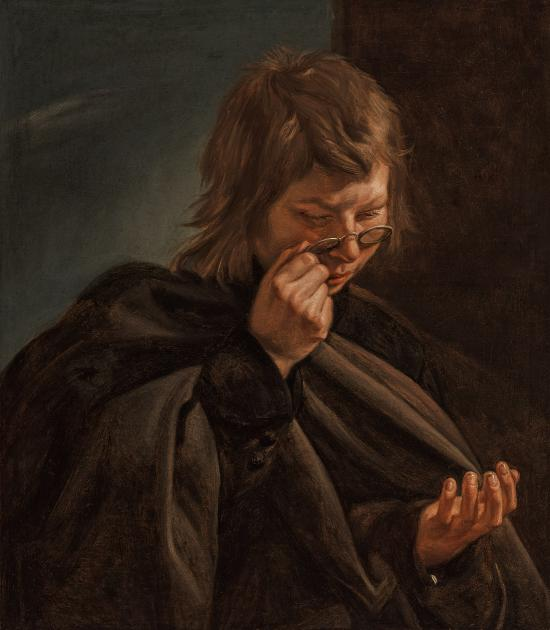
\includegraphics[width=0.75\textwidth]{figs/sight.jpg}
%   \caption{
%       Visualization \#1
%   }
%   \label{fig:Visualization1}
% \end{figure}

% \begin{figure}[ht] 
%   \centering
%   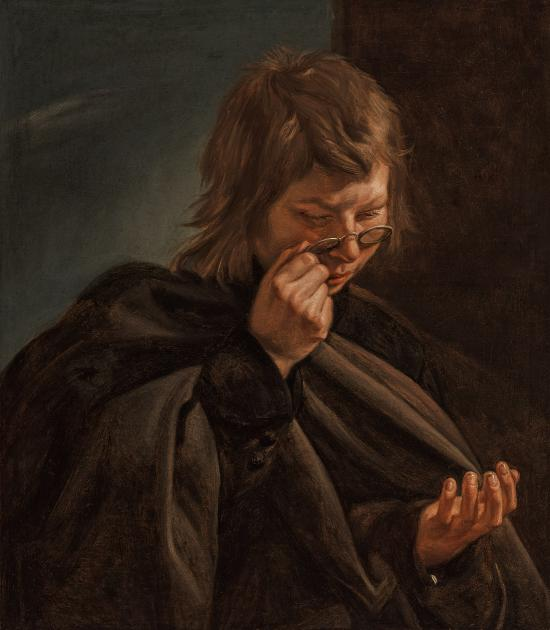
\includegraphics[width=0.75\textwidth]{figs/sight.jpg}
%   \caption{
%       Visualization \#2
%   }
%   \label{fig:Visualization2}
% \end{figure}

\newpage

\section{Report}
\label{sec:sec2}

\subsection{Topic Selection}
\label{subsec:topicSelection}

\subsubsection{Topic Ideation}

For the Misleading visualization I had a few ideas:

\begin{itemize}
  \item Immigration and Crime Correlations: 
  Showing an extrapolated correlation between immigration and crime rates 
  could be made misleading by selecting data points that support a biased narrative.
  For example, not filtering by region, and actively sampling from regions with high crime rates.

  \item Ethnically Biased Drug Usage: 
  Using the "US Drug overdose death rates, by drug type, sex, age, race, and Hispanic origin" 
  \cite{drugOverdoseDeathRates} dataset, we could use missleading bar charts to exaggerate the 
  correlation between hispanic heritage and drug consumption. Additionally, by 
  filtering out specific drugs we could make it especially misleading.

  \item Presidential Employment Claims:
  As much as I do not like Trump, which you'll see in the extra credit,
  the high employment rates during his presidency are largely do to the Covid-19 pandemic.
  We could use a line chart to show the employment rates over time, in contrast/comparison to Biden, 
  and by not clarifying the context of the data, we could make it seem like Trump 
  was solely responsible for the high employment rates.

  \item Immigration Crisis and Democratic Party Correlation:
  We could use a line graph to show the number of border crossings over time, and, by comparing
  Biden's and Trump's presidency, we could make it seem like the Democratic party is solely 
  responsible for the immigration crisis. This could be further exaggerated by not showing the
  Covid-19 pandemic context, and/or picking legal border crossings to be also part of the data using
  the "Border Crossing Entry Data" \cite{borderCrossingEntryData} dataset. 
  
  \item The Cost of Living vs Inflation: 
  The relation between the American people's expenditures, home prices, income, and inflation rates
  are great for generating accurate and misleading content alike. For example, one could
  greatly overvalue the spending power of the American people by not accounting for inflation rates.
  Also, by sampling subsets of the population, we could make homes seem less or more affordable than they are.
\end{itemize}

\subsubsection{Topic Selection and Question}

I decided to go with the "The Cost of Living vs Inflation" topic.

The reason why is because cost of living and income statistics lend themselves to 
both areas of the spectrum of honesty. We can sample and transform numbers 
in multiple ways, incorrecly scale items, and/or dramatize the effects of 
specific economic factors to create missleading narratives 
on the issues americans care most about. This topic also facilities my secondary goal
for this assignment: Showing how changes in data selection and visualization techniques
affect the perception of the viewer.

The question to answer is: 
\textit{Has the increase in home prices made it harder for the average American to own a home?}

I believe that this question will be perfect for evaluating both ends of the spectrum.

We will first try to generate the correct visualization of the data, answering the question
in the most clear and attentive way possible. Then, I aim to generate a visualization 
that creates confusion through various mediums. For example, the missleading visualization 
downplays, exaggerates, or eliminates important considerations like inflation,
and/or misrepresents the increase in home prices through incorrect sampling.

\subsection{Data}
\subsubsection{Required Data}
We will focus on the analysis of yearly data.

The goal was to aquire data regarding:
\begin{itemize}
  \item Home Prices: Real Home Prices, Non-Inflation Adjusted Home Prices, Home Price
  Index data, Rental Prices, Mortgage Prices, or Mortgage Rates.
  \item Income: Real Income, Non-Inflation Adjusted Income, Income Index data, or 
  household earnings.
  \item Miscelaneous: American spending habits and/or miscelaneous expenditures.
\end{itemize}

\subsubsection{Data Gathering}

All data was obtained from the Federal Reserve Economic Data (FRED) database. 

Here is a summary of the specific datasets aquired:

\begin{itemize} 
    
    \item \textbf{Mean Family Income} 
    \begin{itemize} 
      \item \textbf{Series ID}: \texttt{MAFAINUSA646N} 
      \item \textbf{Units}: Current dollars 
    \end{itemize}
  
    \item \textbf{Nominal Median Household Income} 
    \begin{itemize} 
      \item \textbf{Series ID}: \texttt{MEHOINUSA646N} 
      \item \textbf{Units}: Current dollars 
    \end{itemize}

    \item \textbf{Real Median Household Income}
    \begin{itemize}
        \item \textbf{Series ID}: \texttt{MEHOINUSA672N}
        \item \textbf{Units}: Constant dollars (adjusted for inflation)
    \end{itemize}

    \item \textbf{Average Sales Price of Houses Sold}
    \begin{itemize}
        \item \textbf{Series ID}: \texttt{ASPUS}
        \item \textbf{Units}: Current Dollars
    \end{itemize}

    \item \textbf{Median Sales Price of Houses Sold}
    \begin{itemize}
        \item \textbf{Series ID}: \texttt{MSPUS}
        \item \textbf{Units}: Current Dollars
    \end{itemize}

    \item \textbf{Real Residential Property Prices}
    \begin{itemize}
        \item \textbf{Series ID}: \texttt{QUSR628BIS}
        \item \textbf{Units}: Index 2010=100
    \end{itemize}
    
    \item \textbf{Housing Affordability Index}
    \begin{itemize}
        \item \textbf{Series ID}: \texttt{FIXHAI}
        \item \textbf{Units}: Index
    \end{itemize}
    
    \item \textbf{Real Personal Consumption Expenditures}
    \begin{itemize}
        \item \textbf{Series ID}: \texttt{PCEC96}
        \item \textbf{Units}: Billions of Chained 2017 Dollars
    \end{itemize}

    \item \textbf{Personal Consumption Expenditures}
    \begin{itemize}
        \item \textbf{Series ID}: \texttt{PCE}
        \item \textbf{Units}: Billions of Current Dollars
    \end{itemize}
    
    \item \textbf{Retail Sales}
    \begin{itemize}
        \item \textbf{Series ID}: \texttt{RSAFS}
        \item \textbf{Units}: Current dollars
    \end{itemize}

\end{itemize}    

\subsection{Earnest Visualization: Iterative Improvement}
\subsubsection{Understanding The Data}

For the earnest visualization, I want to accurately show whether or not it has become
more difficult for the average american to own a home. 

We have all the necessary data to answer this question, specifically, for plotting the
real wages of the average american against the real home prices.

To eliminate all possible bias, we will use the Real Median Household Income 
and the Real Residential Property Prices datasets. By using the median of household income,
we can avoid the bias of outliers, more accurately showing the average american, 
and, by using the real prices, we can avoid the bias of inflation. 



\subsubsection{Iterative Improvement}

\subsubsection{Visual Encodings}

\subsection{Missleading Visualization: Iterative Deceit}
\subsubsection{Data Obfuscation}
\subsubsection{Iterative Deceit}
The first iteration had a focus on correctly plotting home prices vs real income:
\subsubsection{Effectiveness}

\subsection{Final Designs}
\subsubsection{Do both answer the question?}
\subsubsection{Conclusion}

\newpage
\begin{refcontext}[sorting=nyt]
\printbibliography
\end{refcontext}

\end{document}

